% interactcadsample.tex
% v1.03 - April 2017

\documentclass[]{interact}

\usepackage{epstopdf}% To incorporate .eps illustrations using PDFLaTeX, etc.
\usepackage{subfigure}% Support for small, `sub' figures and tables
%\usepackage[nolists,tablesfirst]{endfloat}% To `separate' figures and tables from text if required

\usepackage{natbib}% Citation support using natbib.sty
\bibpunct[, ]{(}{)}{;}{a}{}{,}% Citation support using natbib.sty
\renewcommand\bibfont{\fontsize{10}{12}\selectfont}% Bibliography support using natbib.sty

\theoremstyle{plain}% Theorem-like structures provided by amsthm.sty
\newtheorem{theorem}{Theorem}[section]
\newtheorem{lemma}[theorem]{Lemma}
\newtheorem{corollary}[theorem]{Corollary}
\newtheorem{proposition}[theorem]{Proposition}

\theoremstyle{definition}
\newtheorem{definition}[theorem]{Definition}
\newtheorem{example}[theorem]{Example}

\theoremstyle{remark}
\newtheorem{remark}{Remark}
\newtheorem{notation}{Notation}

% see https://stackoverflow.com/a/47122900

% Pandoc citation processing

\usepackage{float}
\usepackage[utf8]{inputenc}
\usepackage{subfigure}
\def\tightlist{}
\usepackage[colorlinks=true,
          linkcolor=blue,
          urlcolor=blue,
          citecolor=blue]{hyperref}
\usepackage{booktabs}
\usepackage{longtable}
\usepackage{array}
\usepackage{multirow}
\usepackage{wrapfig}
\usepackage{float}
\usepackage{colortbl}
\usepackage{pdflscape}
\usepackage{tabu}
\usepackage{threeparttable}
\usepackage{threeparttablex}
\usepackage[normalem]{ulem}
\usepackage{makecell}
\usepackage{xcolor}

\begin{document}

\articletype{}

\title{Feasibility study on the use of recycling materials for
prototyping purposes: a comparative study based on the mechanical
resistance}


\author{\name{Victor M. López$^{a}$, Diego Carou$^{b}$, Fabio A. Cruz
S.$^{c, \dagger}$}
\affil{$^{a}$Universidade de Vigo, Departamento de Deseño na Enxeñaría,
Ourense, Spain; $^{b}$University of Jaén, Department of Mechanical and
Mining Engineering, 23071 Jaén, Spain; $^{c}$Université de Lorraine -
ERPI - F-54000, Nancy, France}
}

\thanks{CONTACT Victor M. López. Email: , Diego
Carou. Email: \href{mailto:diecapor@uvigo.es}{\nolinkurl{diecapor@uvigo.es}}, Fabio
A. Cruz
S.. Email: \href{mailto:cruzsanc1@univ-lorraine.fr}{\nolinkurl{cruzsanc1@univ-lorraine.fr}}}

\maketitle

\begin{abstract}
The development of 3D printing is seen as a disruptive technology and
continues to expand the boundaries of design space for manufacturing
prototypes and final products. However, nowadays the sustainability is
one of the major objectives for manufacturing and the use of recycled
materials becomes a suitable strategy when economic, environmental and
technical feasibility are verified. 3D printing is still a novel
manufacturing process and the research on the topic is still limited,
particularly when referring to improve resource efficiency issues. This
paper attempts to evaluate the suitability of the substitution of virgin
polylactic acid (PLA) by recycled PLA. To do that, it includes an
experimental plan divided into three phases to evaluate the mechanical
resistance. The results showed that recycled PLA may be used due to the,
though slightly lower, similar mechanical resistance than that of the
virgin material. This reduction is limited to 13 \% in the worst
configuration (vertical). Besides, it was identified how the infill
density and the orientation used for printing played a major role on the
mechanical resistance, when others such as the infill pattern, printing
speed and layer height had non-significant influence. It was found that
there is a retention of the 58.1\% of the mechanical resistance using an
infill density of 40\%. This is a relevant insight for prescriptions of
the 3D printing parameters guaranteeing minimal quality conditions in
the prototyping phases.
\end{abstract}

\begin{keywords}
Prototyping;
\end{keywords}

\hypertarget{introduction}{%
\section{Introduction}\label{introduction}}

Additive manufacturing (also called 3D printing) is becoming a key
technology for cross domain applications. The layer-by-layer principle
of manufacturing objects enables a higher flexibility degree in the
product design phase. The set of several available printing technologies
is pushing forward advantages such as the customization of objects with
complex geometries with a great deal of detail, combination of different
materials \citep{Askari2020}, reduction of the need for assembly and
high utilization rate of raw materials \citep{Perez2020, Wang2020f}.
Thus, this field is receiving great attention by the industrial
companies and the general public.

3D printing has developed significantly over time. A great development
is expected in sectors such as product consumption, medical products and
aerospace components \citep{Peng2018}. The rapid prototyping market
reached \$11.86 billion US dollars according to Wohlers 2019 report
\citep{Singh2021}, which also forecasts the market to reach 35.6 billion
dollars by 2024 \citep{Forbes2020}.

Nowadays, there is a need to find paths to reduce the ecological impact
of manufacturing processes and activities \citep{Niaki2019}. Researchers
are making efforts to identify opportunities of 3D printing on the
circular economy paradigm \citep{Despeisse2016}. Moreover, due to the
fact that plastic is one of the most used materials in the 3D printing
industry \citep{GonzalezHenriquez2019}, and given their
non-biodegradable nature, plastic is one the most abundant type of waste
produced and their impact is well document in the different ecosystems
\citep{Ryberg2019}. Thus, reducing the consumption of plastics is of
great importance for the environment.

A major literature coming from engineering, human computer interaction,
design thinking or software development \citep{Elverum2016a} validates
the rationale for the prototyping phase in the early design phases of
product development. According the prototyping theory, different kind of
prototypes are needed during the new product development phases (eg.
prototype for desirability, for feasibility, and for viability)
\citep{Menold2017} with the purpose of reducing uncertainties, exploring
new ideas, increasing feasibility and/or engaging with users
\citep{Hansen2020}. Based on that, a prototype is accomplished in terms
of certain aims: (1) Model to Link, (2) Model to Test, (3) Model to
Communicate, (4) Model to Decide, and (5) Model to Interact
\citep{Menold2017}. The use of digital tools allows designers to create
highly flexible prototypes that enable short learning cycles at an
affordable cost. Moreover, the use of 3D printing technology enables the
materialization aspect. Regardless of whether the printed part is
functional or not, the printed part is found to be valuable in design
decisions \citep{Elverum2016}. However, there is a gap in the literature
in terms of sustainable manufacturing using 3D printing in the early
design phases \citep{Peng2018}. Although the technology offers high
efficiency in the use of material, the democratization of this
technology could cause a rebound impact due to the increasing generation
and disposal of huge amounts of waste or polluting emissions to
fabricate the virgin feedstock required, particularly, in the
prototyping phases. Without a doubt, the roots of FFF (Fused Filament
Fabrication) are linked to the rapid prototyping concept
\citep{Campbell2012, Bourell2009} and in the last years it has been
widely adopted by industry, academia and users to create functional
objects for their designs. Therefore, one question that remains is how
to define the most favorable printing conditions in order to create
prototypes in the early phases without compromising the mechanical
properties, even for recycled feedstocks.

Studies on the technical viability of recycled materials as substitutes
for conventional virgin materials are still limited for particular
applications \citep{CruzSanchez2020}. It is important to note that in
most cases, prototypes do not require excellent mechanical resistance
but the minimum to be handled in order to allow inspection and
measurement. Thus, the type of material used and its amount can be
further optimized when it comes to prototyping.

The present study evaluates the mechanical properties of both
conventional and recycled polylactic acid (PLA) materials. The objective
is the assessment of the suitability of the recycled PLA as replacement
in prototyping, though its use may be further extended to other
applications. To do that, this research is based on a comprehensive
experimental study with three main phases in order to evaluate the
influence of several printing parameters on the mechanical properties of
the parts. In section \ref{section:background}, a literature review is
presented, focusing on the critical parameters in 3D printing technology
and providing readers with an overview on the use of a distributed
recycling approach. Then, section \ref{section:experimental} illustrates
the methodology used in this study. In section \ref{section:findings},
the results of the experimental approach is presented. In section
\ref{section:discussion}, we discuss the main research outcomes.
Finally, section \ref{section:conclusions} summarizes the main
conclusions.

\hypertarget{existing-theories-previous-work}{%
\section{Existing Theories \& Previous
Work}\label{existing-theories-previous-work}}

\label{section:background}

\hypertarget{main-parameters-on-fused-filament-fabrication}{%
\subsection{Main parameters on Fused Filament
Fabrication}\label{main-parameters-on-fused-filament-fabrication}}

One of the most common processes in 3D printing is the FFF (also known
as fused deposition process modeling (FDM), which is a trademark). The
process is based on material extrusion, so the material is heated above
its melting point and then deposited onto a platform
\citep{Wolszczak2018}. In FFF/FDM, a variety of thermoplastic materials
are commonly used, such as acrylonitrile butadiene styrene (ABS),
polyvinylchloride (PVS), polycarbonate (PC), nylon, polifenilsulfona,
high density polyethylene (HDPE), low density polyethylene (LDPE),
polyethylene terephthalate (PET), high impact polystyrene (HIPS) and
polylactic acid (PLA) \citep{Chua2017, Zhao2018a, Singh2018e}.

The mechanical properties are critical for engineering parts,
particularly, for 3D printed because of the anisotropic behaviour, which
can influence up to about 47\% the ultimate tensile strength in function
of the manufacturing parameters \citep{Laureto2018}. Using a systematic
literature review, \citet{Popescu2018} identified certain key parameters
influencing the printed parts including raster-to-raster air gap, raster
angle, layer thickness, infill density and build orientation.\\
Nevertheless, it is highlighted that it might be uncertain if a set of
optimal parameters for a machine/material/application combination can be
transferred to other 3D printers due to the issue of intra-3D printer
variability. The development of standards to qualify the process is a
relevant research path in order to set minimal requirements for the
dimensional accuracy, repeatability and minimum feature size among the
3D printing technologies \citep{Rebaioli2017}. Likewise, considering the
open source nature of the FFF technology, standardized experimental
protocols are relevant to enable benchmarking and serve as a guide for
machine selection \citep{CruzSanchez2014, Roberson2013}. Therefore, it
is crucial to identify the most important parameters that may affect the
response variable among all of the available to carry out the process
and their expected influence based on the scientific literature
\citep{JaisinghSheoran2019}.

In general terms, it is found that for low values of layer height, the
tensile strength of the material is improved \citep{Tymrak2014a}. In
addition, by directing the printing towards the direction in which the
tensile load will be applied during tensile testing, the property can be
also maximized. The importance of the printing orientation was also
identified by \citet{Yao2019}. According to \citet{Alafaghani2018}, a
higher extrusion temperature, an optimized layer thickness, a triangular
filling pattern and a higher filling level maximize the strength of the
parts. Regarding the printing speed, it is identified that higher
printing speed with higher layer thickness leads to lower part strength.
Among others, \citet{Altan2018} also identified the influence of the
layer height on the mechanical resistance.

\hypertarget{materials-and-distruted-recycling}{%
\subsection{Materials and distruted
recycling}\label{materials-and-distruted-recycling}}

The development of new materials such as polymers, elastomers and
composites in engineering plays a fundamental role in the advance of
sustainable manufacturing \citep{Ashby2013}. \citet{Liu2019a} presented
a complete review on natural-derived biopolymers for 3D printing
purposes, with a particular focus on biomedical, customized food
fabrication and textile and apparel products. They pointed out that the
use of biopolymers of natural and renewable origin, replacing synthetic
polymers, as the cellulose, hemicellulose, lignin, starch, alginate,
chitosan and derivatives, represents the most abundant bio-based and
renewable raw materials for different 3D printing technologies.

Polylactic acid (PLA) is a type of natural biopolymer obtained from
crops such as starch or sugar cane. It is a biodegradable biopolymer
consisting of lactic acid molecules and it is one of the most used
materials in 3D printing. In addition, PLA is a sustainable alternative
that shows a range of crystallinity and mechanical properties between
polystyrene and polyethylene terephthalate
\citep{Kumar2018b, Zhao2018a}.

In the literature, the distributed recycling via additive manufacturing
approach (DRAM) makes an emphasis in the technical steps to reuse
plastic waste through the recycling chains for material extrusion based
3D printing \citep{CruzSanchez2020, Little2020}. The use of recycled
material as raw material or blended with virgin material is a method of
special interest to contribute to manufacture in a sustainable way
\citep{Zhao2018}. In the DRAM methodology, consumers have an economic
incentive to recycle. This is because they can use their waste as
feedstock for a wide range of consumer products that can be produced for
a fraction of the conventional cost of the equivalent products.
Moreover, 3D printing is especially suited because it allows producing
parts with (almost) no waste and could reduce more than 40\% of the
waste related to the material, reusing 95\% of the unused material
\citep{Petrovic2011}. Currently, most of the cost of 3D printing is
associated with the cost of the filament \citep{Wittbrodt2013}. By
recycling raw materials such as PLA, the emissions of carbon dioxide can
be reduced in the transport to landfills or shipping to customers
offering environmental benefits \citep{Santander2020}. The technical
feasibility for recycling in laboratory conditions have been proved for
PLA \citep{CruzSanchez2017}, ABS \citep{Vidakis2020} and PET
\citep{Zander2018}, finding that the recycled plastics have a similar
performance to their virgin counterparts and they have even been applied
in the manufacture of high value products in some sectors such as the
automobile \citep{Zhao2018}.

It is important to evaluate the properties of the recycled materials
before substituting virgin for recycled materials. In this sense,
\citet{Kumar2018b} compared the elongation at break, load at break, flow
index, Young's modulus and breaking stress of recycled ABS, high impact
polystyrene (HIPS) and PLA. The PLA showed the highest elongation at
break along with the ABS. In addition, the PLA had a higher breaking
load and breaking stress, although a smaller Young's modulus. Other
authors such as \citet{Gu2016} identified the suitability of using
recycled polypropylene instead of virgin polypropylene based on
mechanical properties. Specifically, they found that the use of fillers
(talc and glass fibre) improved the mechanical properties.
\citet{Babagowda2018} studied the influence of the percentage of
recycled PLA used in the filament (i.e., 10 to 50 \%) showing that the
smaller the percentage the higher the ultimate tensile strength.
\citet{Pinho2020} obtained higher values of tensile stress for recycled
PLA when comparing to the virgin one.

As \citet{Suarez2020} pointed out, the use of recycled materials is
still uncertain because of the potential changes in the material
properties when recycling. \citet{Zhao2018} studied the cycles of
printing that PLA can withstand until it loses much of its properties.
Thus, they showed that PLA adequately withstands two printing cycles
since in a third cycle the mechanical properties and viscosity decreased
considerably. The increase in crystallinity and melting enthalpy and the
decrease of the cold crystallization enthalpy are attributed to the 3D
printing process, not to the recycling performed by the extrusion
process. Similarly, other authors such as \citet{Lanzotti2019} have
proved how recycling PLA provides comparable mechanical properties as
the virgin material only after a second recycling process.

The recycling of PLA has certain limitations because of reducing the
molecular weight with its reuse, resulting in degradation and decrease
of mechanical properties. To counteract this effect, it is possible to
add polidopamine (PDA) on the surface to improve these properties.
Viscosity is also reduced with each printing cycle, but it could be
corrected by adding virgin plastic \citep{Zhao2018, Zhao2018a}. When
recycling, there is a decrease in the properties of the material as a
result of the presence of carbonyl groups and superficial pitting due to
thermomechanical degradation during the new melting process that takes
place during 3D printing \citep{Zhao2018}.

It is found that this valuable literature is focused on the evaluation
and optimization of printed parts that seek the best trade-offs among
parameters for a final product. The aim of the study is to identify the
major critical factors affecting the mechanical properties in FFF
focusing prototyping purposes, evaluating their impact on the mechanical
properties, particularly for both virgin and recycled PLA. Thus, based
on the results, it is expected to gain a better understanding on the
suitability of using recycled materials in 3D printing and how to
properly select the printing conditions to guarantee sufficient
mechanical resistance in prototypes. In order to do that, an
experimental plan comprising three phases will be developed. This is a
complementary approach to the well established literature on FFF.

\hypertarget{experimental-procedure}{%
\section{Experimental procedure}\label{experimental-procedure}}

\label{section:experimental}

\hypertarget{materials-and-equipment}{%
\subsection{Materials and equipment}\label{materials-and-equipment}}

The printing materials tested in the study were virgin and recycled PLA
characterized by data listed in Table \ref{tab:table1}. Both materials
were commercial ones, the recycled PLA contained 10 \% of virgin PLA in
the blend.

\begin{table}[H]

\caption{Characterization and processing conditions of the used PLA and recycled PLA. \label{tab:table1}}
\centering
\begin{tabular}[t]{l>{\raggedright\arraybackslash}p{4.5cm}>{\raggedright\arraybackslash}p{4.5cm}}
\toprule
 & PLA & Recycled PLA\\
\midrule
\cellcolor{gray!6}{Composition} & \cellcolor{gray!6}{PLA (Polylactic resin)- 99\% CAS: 9051-89-2} & \cellcolor{gray!6}{PLA - 10\% CAS: 9051-89-2 and recycled PLA 90\%}\\
Density & 1.24 g/$cm^{3}$ & 1.1-1.3 $cm^{3}$\\
\cellcolor{gray!6}{Diameter} & \cellcolor{gray!6}{1.75 ± 0.03 mm} & \cellcolor{gray!6}{1.75 mm}\\
Printing temperature & 220 ± 20 ºC & 205 ± 15 ºC\\
\cellcolor{gray!6}{Melting temperature} & \cellcolor{gray!6}{180 ºC} & \cellcolor{gray!6}{160 ± 10 ºC}\\
\bottomrule
\end{tabular}
\end{table}

The specimens were printed with a BQ's Witbox, shown in Fig. 1a. The
software used to generate the printing code was the Ultimaker Cura
3.2.1. To perform the destructive test, the machine used was the MTS
Criterion 43 universal testing machine (MTS, 2020) (Fig 1b) with a
maximum load of 50 kN, being the maximum load supported by the LPS 104
cell of 10 kN. The clamping system was the Instron 2716-015 system with
a maximum supported load of 30 kN. The selected strain rate was 0.5
mm/min.

In this study, the mechanical specimens were manufactured according to
the dimensions proposed by \citet{Lin2018} in which the length of the
specimen was 75 mm. The dimensions of the specimen are the ones depicted
in Fig 1c.

\begin{figure}

{\centering 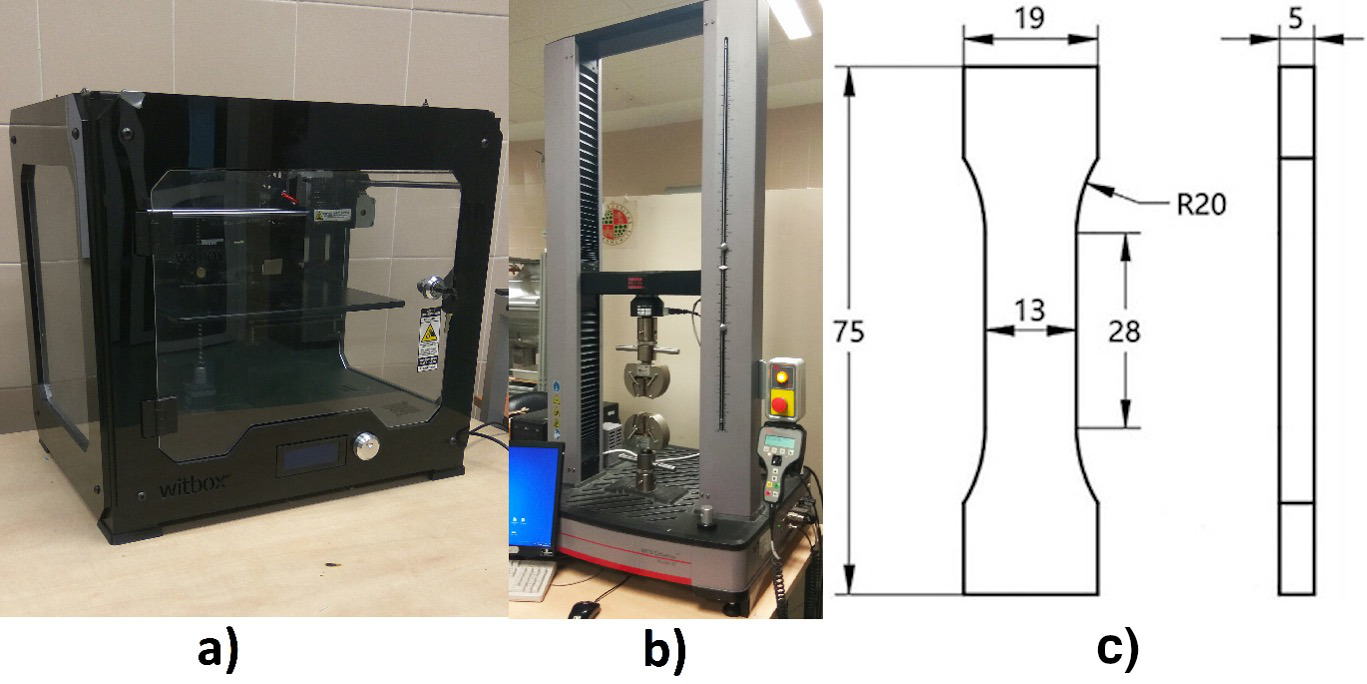
\includegraphics[width=0.9\linewidth]{Figures/Machine-probeta} 

}

\caption{Equipment used in the study: a) 3D printer, b) Universal testing machine an c) mechanical sample.}\label{fig:Fig.machine}
\end{figure}

\hypertarget{methodology}{%
\subsection{Methodology}\label{methodology}}

Fractional designs are useful for minimizing the number of tests,
reducing time and money \citep{Montgomery2001}, being used as screening
designs. Hence, the experimental plan included three different phases
(Figure \ref{fig:methodology}) to carry out a comprehensive study with a
limited number of tests that do not compromise the reliability of the
results using fractional designs.

The main goal of \emph{Phase I} is to identify and discard factors
depending on their influence on the response variable. The response
variable chosen was the maximum load attained during the testing of the
specimen \citep{Kumar2018b, Chacon2017, Letcher2015}. In this phase, the
design included only a specimen printed in the horizontal orientation
for each of the combinations, not evaluating the influence of the
orientation. The use of random order allowed guaranteeing that the
hypothesis that the errors are independently distributed random
variables was fulfilled \citep{Montgomery2001}. Based on the literature
research presented in section \label{section:background}, the critical
parameters for the study are the (1) layer height -LH- and (2) infill
pattern -IP-. In addition, taking into account the goal of sustainable
manufacturing (i.e., trying to optimize the consumption of material),
but also productivity (i.e., trying to minimize printing times), (3)
infill density -ID- and (4) printing speed -PS- were considered
\citep{Singh2019, Tanveer2019}. These four factors were selected using
two levels for each of them with large ranges. In consequence, the
factors and their levels were: layer height -LH- (0.15 and 0.3 mm),
infill pattern -IP- (tri-hexagonal and grid), infill density -ID- (60
and 100 \%) and printing speed -PS- (40 and 80 mm/s). The selected
printing temperature was 210 °C, which was the recommended for PLA
material. This phase ends with an analysis of variance (ANOVA) in order
to identify the influential factors on the response variable.

Then, the main goal of \emph{Phase II} is to study in more detail the
influence of the most influential factor according to the \emph{Phase
I}. Thus, the intent is to make a focus on how the response variable
evolves by varying the most influential factor. For that reason, in this
phase an extension of the factor levels was established. On the other
hand, the criteria selection of levels for the other three factors aimed
at minimizing the printing time.

Finally, the \emph{Phase III} aimed at evaluating the influence of the
anisotropy of the specimens based on the study of the printing
orientation, which may notably affect the mechanical resistance. In this
phase, the main focus is to analyse the influence of the building
orientation. Because of the anisotropy, the UNE 116005:2012 \citep{UNE}
standard requires printing the specimens in three different
orientations: edgewise (E), horizontal (H) and vertical (V), testing
five samples in each orientation. This phase included the printing of 15
specimens of both virgin and recycled PLA.

\begin{figure}

{\centering 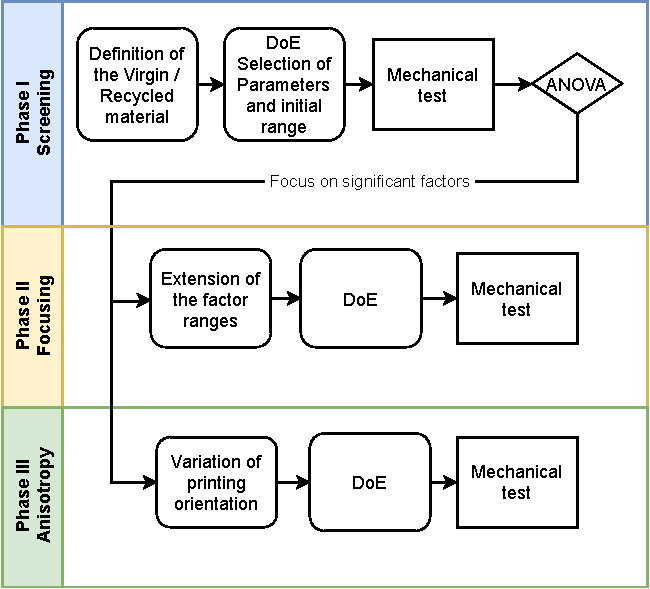
\includegraphics[width=0.7\linewidth]{Figures/Methodology} 

}

\caption{Summary of the three phases of the experimental plan.\label{fig:methodology}}\label{fig:Fig.Methodology}
\end{figure}

\hypertarget{findings}{%
\section{Findings}\label{findings}}

\label{section:findings}

\hypertarget{phase-i-screening-phase}{%
\subsection{Phase I: Screening phase}\label{phase-i-screening-phase}}

Table \ref{tab:phase1} summarizes the experimental strategy with the
results of the maximum load attained during this screening phase. A
total of 16 samples were tested.

\begin{table}

\caption{\label{tab:table.S2}Results of the Phase 1. \label{tab:phase1}}
\centering
\fontsize{7}{9}\selectfont
\begin{threeparttable}
\begin{tabular}[t]{lllrrr}
\toprule
Material & LH (mm) & IP & ID (\%) & PS (mm/s) & Max Load (kN)\\
\midrule
\cellcolor{gray!6}{Virgin} & \cellcolor{gray!6}{0.15} & \cellcolor{gray!6}{Tri-hex} & \cellcolor{gray!6}{60} & \cellcolor{gray!6}{40} & \cellcolor{gray!6}{2.21}\\
Virgin & 0.3 & Tri-hex & 60 & 80 & 2.16\\
\cellcolor{gray!6}{Virgin} & \cellcolor{gray!6}{0.15} & \cellcolor{gray!6}{Grid} & \cellcolor{gray!6}{60} & \cellcolor{gray!6}{80} & \cellcolor{gray!6}{2.24}\\
Virgin & 0.3 & Grid & 100 & 80 & 3.60\\
\cellcolor{gray!6}{Virgin} & \cellcolor{gray!6}{0.3} & \cellcolor{gray!6}{Tri-hex} & \cellcolor{gray!6}{100} & \cellcolor{gray!6}{40} & \cellcolor{gray!6}{3.62}\\
Virgin & 0.15 & Tri-hex & 100 & 80 & 3.81\\
\cellcolor{gray!6}{Virgin} & \cellcolor{gray!6}{0.15} & \cellcolor{gray!6}{Grid} & \cellcolor{gray!6}{100} & \cellcolor{gray!6}{40} & \cellcolor{gray!6}{3.79}\\
Virgin & 0.3 & Grid & 60 & 40 & 2.16\\
\cellcolor{gray!6}{Recycled} & \cellcolor{gray!6}{0.15} & \cellcolor{gray!6}{Tri-hex} & \cellcolor{gray!6}{60} & \cellcolor{gray!6}{40} & \cellcolor{gray!6}{2.16}\\
Recycled & 0.3 & Tri-hex & 60 & 80 & 2.16\\
\cellcolor{gray!6}{Recycled} & \cellcolor{gray!6}{0.3} & \cellcolor{gray!6}{Grid} & \cellcolor{gray!6}{60} & \cellcolor{gray!6}{40} & \cellcolor{gray!6}{2.15}\\
Recycled & 0.15 & Tri-hex & 100 & 80 & 3.38\\
\cellcolor{gray!6}{Recycled} & \cellcolor{gray!6}{0.3} & \cellcolor{gray!6}{Tri-hex} & \cellcolor{gray!6}{100} & \cellcolor{gray!6}{40} & \cellcolor{gray!6}{3.37}\\
Recycled & 0.15 & Grid & 60 & 80 & 2.05\\
\cellcolor{gray!6}{Recycled} & \cellcolor{gray!6}{0.15} & \cellcolor{gray!6}{Grid} & \cellcolor{gray!6}{100} & \cellcolor{gray!6}{40} & \cellcolor{gray!6}{3.53}\\
Recycled & 0.3 & Grid & 100 & 80 & 3.49\\
\bottomrule
\end{tabular}
\begin{tablenotes}
\item \textit{Note: } 
\item Layer height (LH), Infill pattern (IP), Infill density (ID), Printing speed (PS)
\end{tablenotes}
\end{threeparttable}
\end{table}

In general, shortly after attaining the maximum load, the fracture of
the specimen occurred. However, the nature of the fracture was not
homogeneous as shown in Fig \ref{Fig:Phase.1a}. Thus, in most cases, the
specimens showed a fragile behavior and the fracture, either
horizontally or with a lower inclination angle, was clean. However, for
the recycled material, the specimens presented a ductile behavior and,
properly, the fracture did not occur after the maximum load was
attained. In these cases, the tensile tests were cancelled after the
maximum load was attained, without reaching a complete fracture of the
specimen. The breakage in these cases occurred at a 45º angle and, in
the case of the RE-2 specimen, two parallel fracture lines can be
clearly seen. The images of the fractured specimens did not allow us to
observe a clear relation of the fracture of the specimens to the
printing conditions. However, the fracture behavior may relate to that
explained by \citet{Yao2019}. The authors identified two different types
of fracture: in-layer and interlayer. In general, the interlayer
fracture occurs at the interface of two layers when printing in vertical
position, even when varying the printing orientation up to 45º from the
vertical position. In-layer fracture is more likely when the specimen is
printed using an edgewise position (or, inclined up to 45º from that
position). In this case, the printing direction is the same as the
tensile stress direction, which also happens when the horizontal
orientation is used. In these cases, the material layer is not intact
after the fracture. As a result, it is likely that both modes (in-layer
and inter-layer fractures) coexist in this study, which may explain the
heterogeneity of the different fractures.

\begin{figure}[!t]
\centering
\subfigure[Tensile sample of the Phase 1]{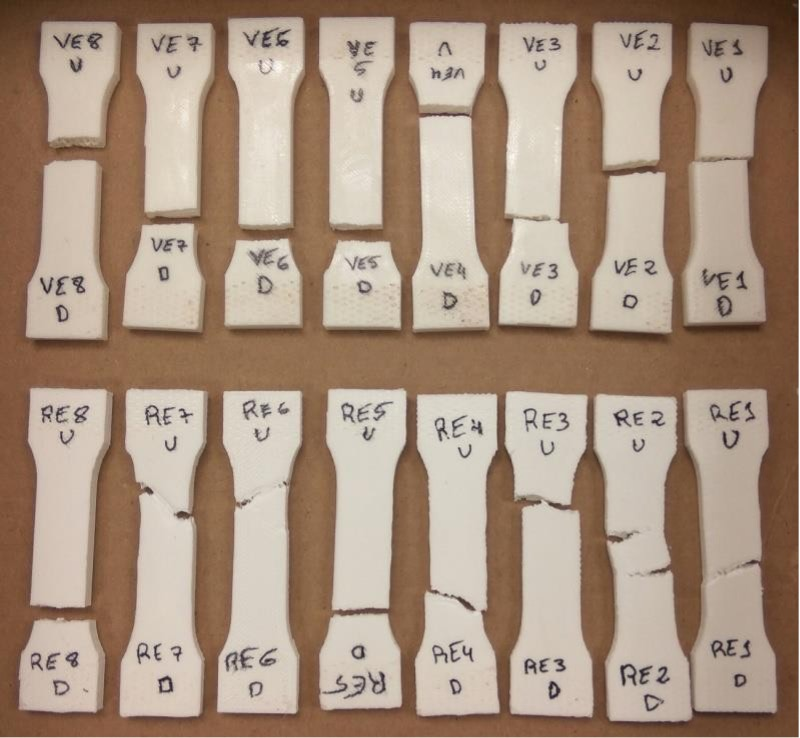
\includegraphics[width=0.49\linewidth]{Figures/Probetas-Fase-1.jpg}%
\label{Fig:Phase.1a}}
\hfill
\subfigure[Boxplots to identify significant factors based on DoE]{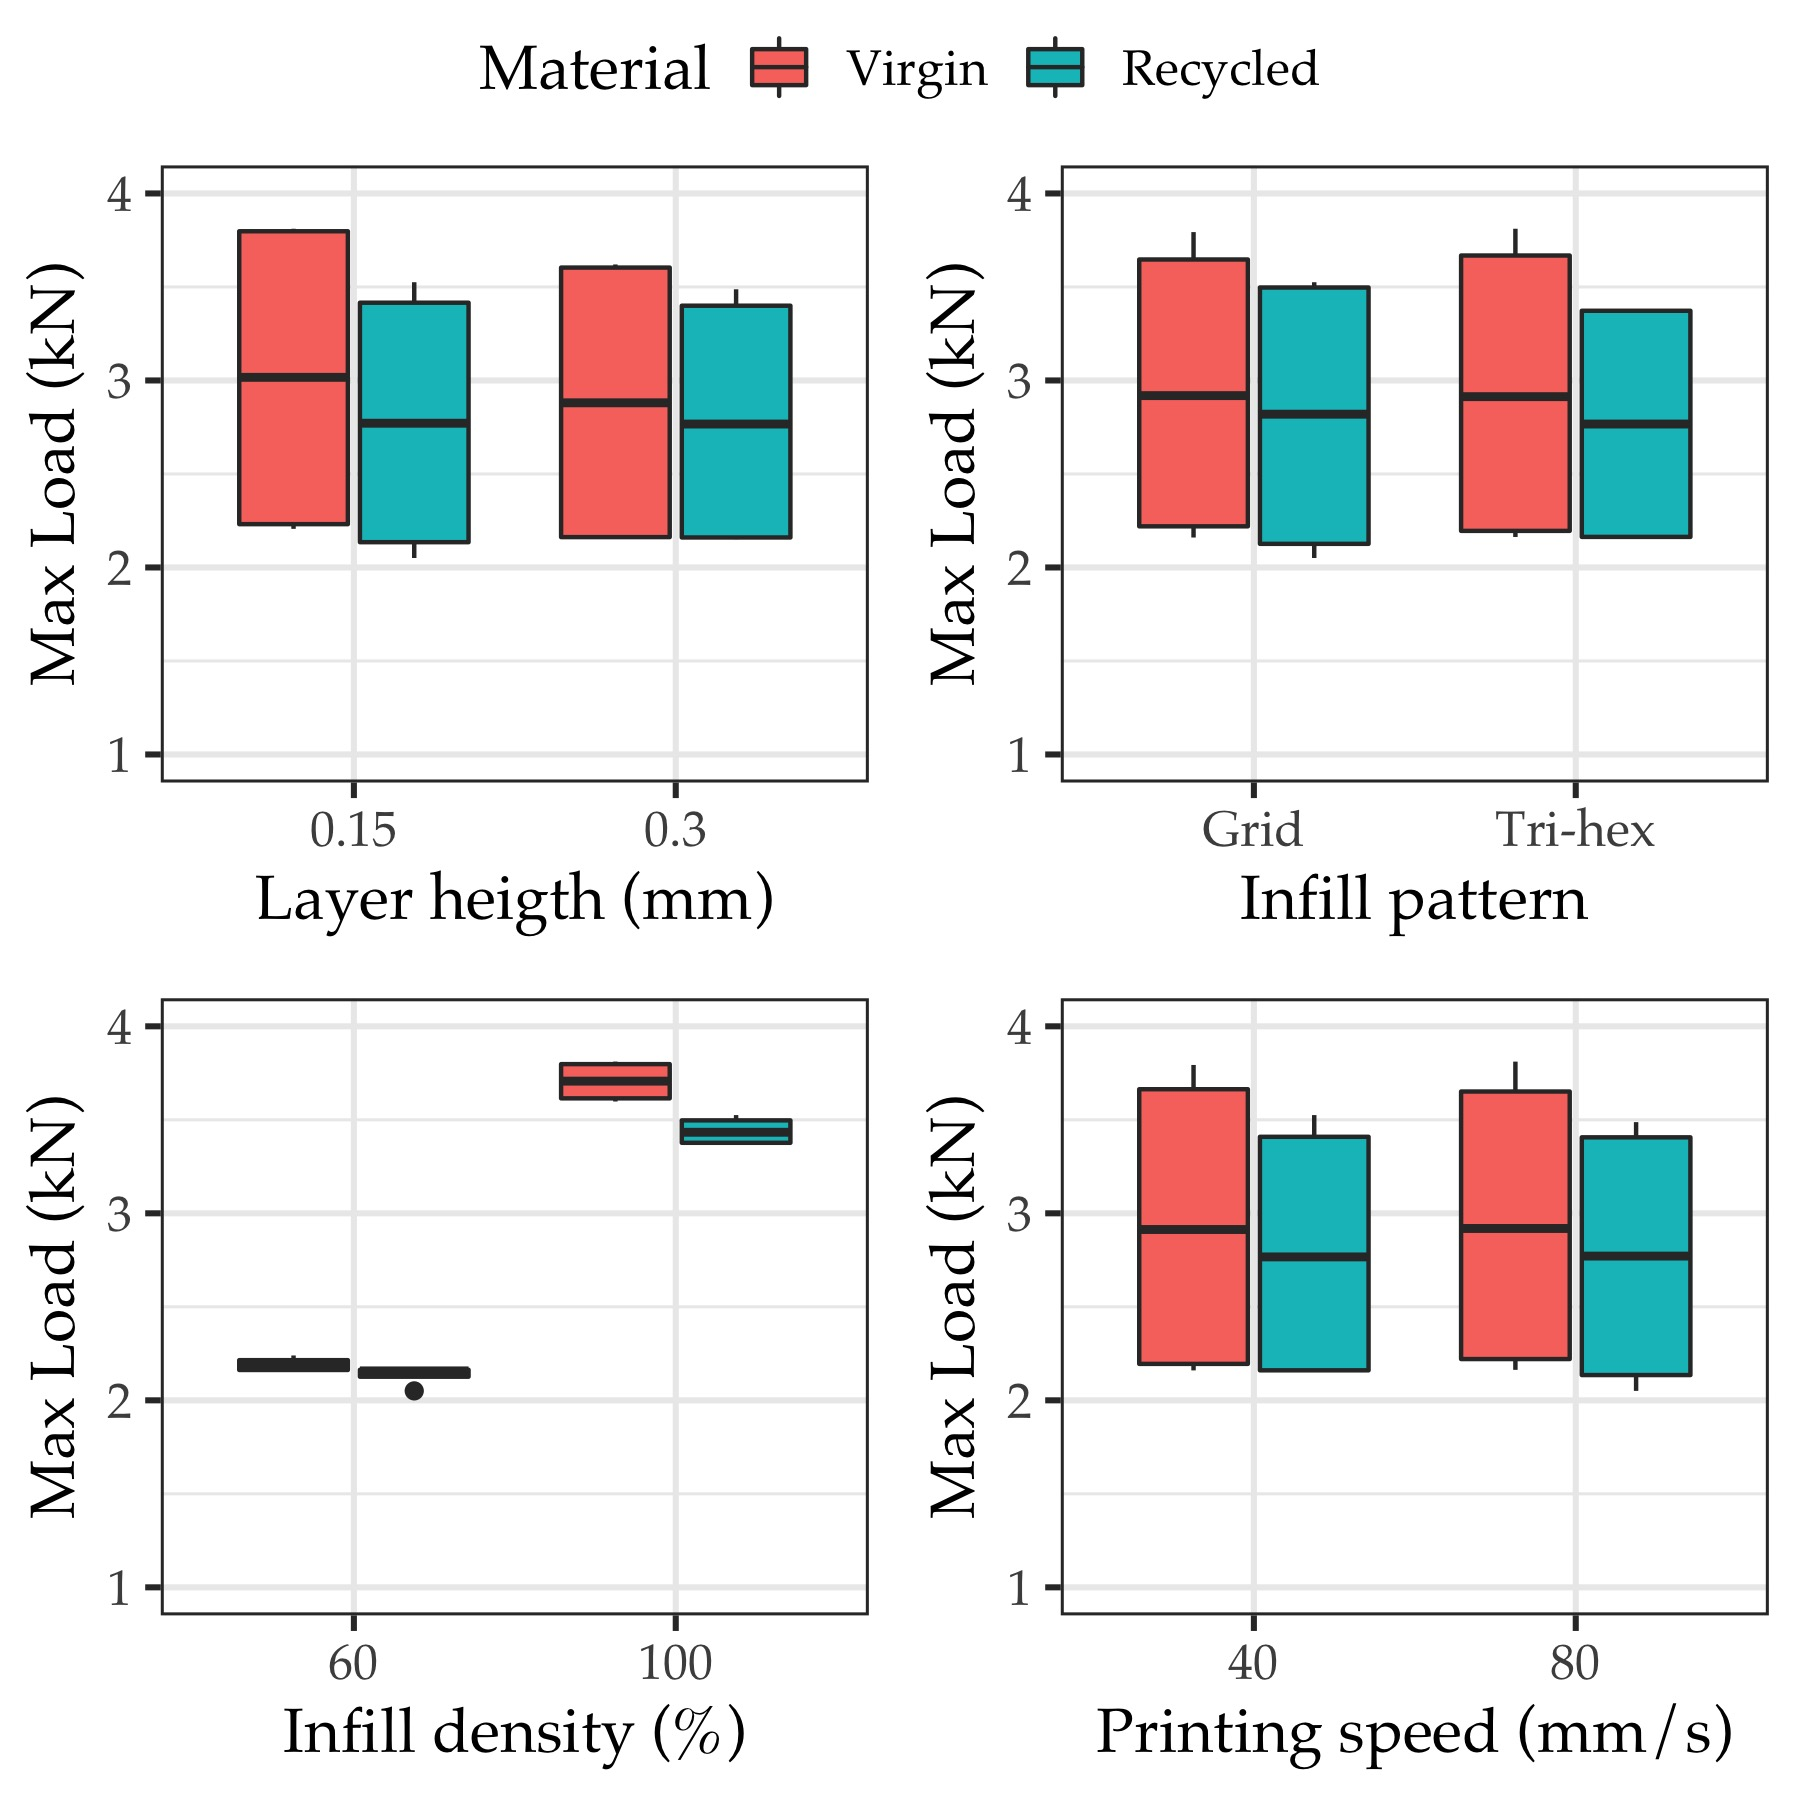
\includegraphics[width=0.49\linewidth]{Figures/Phase-1-2.jpg}%
\label{Fig:Phase.1b}}
\caption{Phase 1: screening tests to identify significant factors based on DoE}
\end{figure}

An analysis of variance (ANOVA) was performed using R software in order
to identify the influential factors on the response variable. As
criterion, critical factors for the response variable were those with
p-values lower than 0.05 \citep{Perez2018}. Shapiro-Wilk normality tests
allowed verifying the normality of the residuals. The figure
\ref{Fig:Phase.1b} illustrates the boxplots of the results considering
each of the factors. Also, the Table \ref{tab:anova.phase1} lists the
results of the ANOVAs carried out for the experimental results.

\begin{table}

\caption{\label{tab:Table.Anova.fase1}ANOVA results at 95\% significance level \label{tab:anova.phase1}}
\centering
\begin{tabular}[t]{llllll}
\toprule
  & Df & Sum Sq & Mean Sq & F value & Pr(F)\\
\midrule
\cellcolor{gray!6}{LH} & \cellcolor{gray!6}{1} & \cellcolor{gray!6}{0.0129} & \cellcolor{gray!6}{0.0129} & \cellcolor{gray!6}{1.34} & \cellcolor{gray!6}{0.274}\\
IP & 1 & 0.00104 & 0.00104 & 0.107 & 0.75\\
\cellcolor{gray!6}{ID} & \cellcolor{gray!6}{1} & \cellcolor{gray!6}{7.96} & \cellcolor{gray!6}{7.96} & \cellcolor{gray!6}{825} & \cellcolor{gray!6}{6.1e-11***}\\
PS & 1 & 0.000601 & 0.000601 & 0.0623 & 0.808\\
\cellcolor{gray!6}{Material} & \cellcolor{gray!6}{1} & \cellcolor{gray!6}{0.106} & \cellcolor{gray!6}{0.106} & \cellcolor{gray!6}{11} & \cellcolor{gray!6}{0.00788**}\\
Residuals & 10 & 0.0965 & 0.00965 &  & \\
\bottomrule
\multicolumn{6}{l}{\rule{0pt}{1em}\textit{Note: }}\\
\multicolumn{6}{l}{\rule{0pt}{1em}Signif. codes:  0 ‘***’ 0.001 ‘**’ 0.01 ‘*’ 0.05 ‘.’ 0.1 ‘ ’ 1}\\
\end{tabular}
\end{table}

From the results of the Table \ref{tab:anova.phase1} and figure
\ref{Fig:Phase.1b}, it can be clearly identified how the infill density
was a statistically significant factor for the maximum load with the
lowest p-value, lower than 0.001, among the studied factors. Likewise,
the type of material is also a statistically significant factor for the
response variable but with a higher p-value, being non-significant the
rest of the factors. When evaluating the contribution of each of the
factors to the variability explained by the model, there were calculated
values of 97.3\% and 1.3\% for infill density and type of material,
respectively. Thus, when manufacturing new parts or specimens, infill
density is a key factor for guaranteeing adequate mechanical properties
of the specimens.

\hypertarget{phase-ii-focusing}{%
\subsection{Phase II: Focusing}\label{phase-ii-focusing}}

The main goal of \emph{Phase II} is the detailed evaluation of the
infill density by the fact that it was observed as the most important
factor affecting the mechanical resistance in the previous phase.
Therefore, five levels of the infill density were chosen ranging from 40
to 100 \% to evaluate the evolution of the maximum load for both virgin
and recycled PLA. The specific levels selected were 40, 55, 70, 85 and
100 \%. Regarding the selection of the other factors of the printing
process, the main criteria was the reduction of the printing time as
stated in the methodology section. Therefore, the experimental
conditions were layer height of 0.3 mm, tri-hexagonal infill pattern and
printing speed of 80 mm/s with an estimated printing time of 20 min. A
total of 10 samples were manufactured.

\begin{figure}[!t]
\centering
\subfigure[Specimens after tensile test in  phase II]{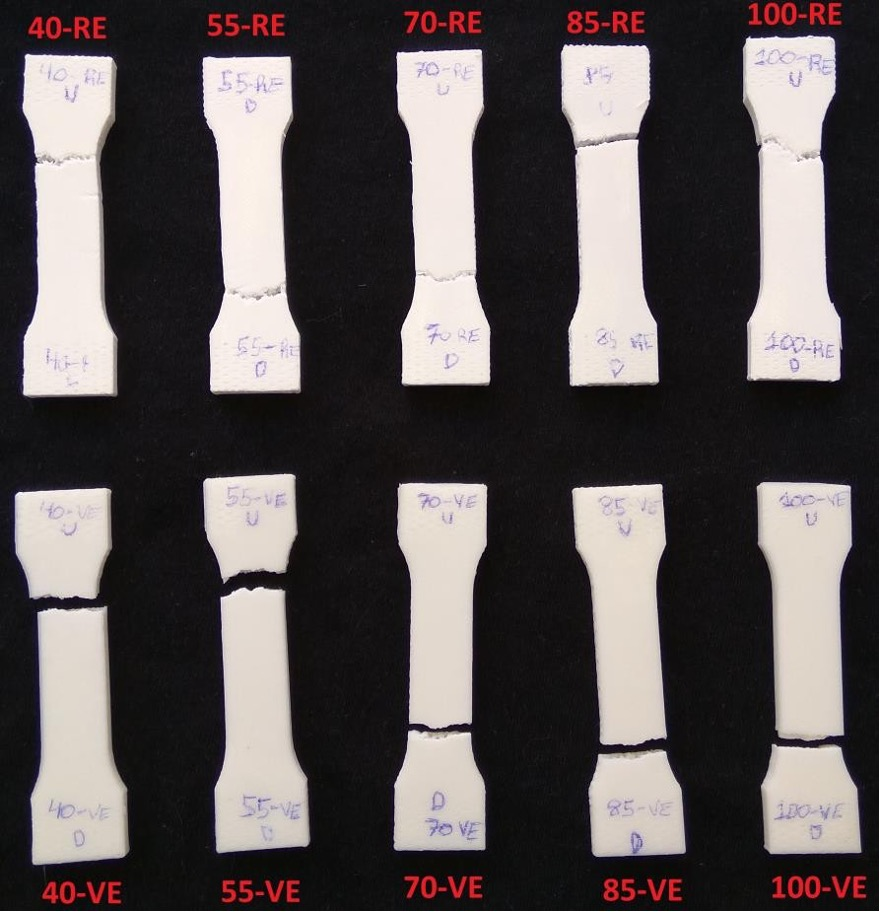
\includegraphics[width=0.49\linewidth]{Figures/Probetas-Fase-2.jpg}%
\label{fig:probetas.phase2}}
\hfill
\subfigure[Maximum load versus infill density for both virgin and recycled PLA.]{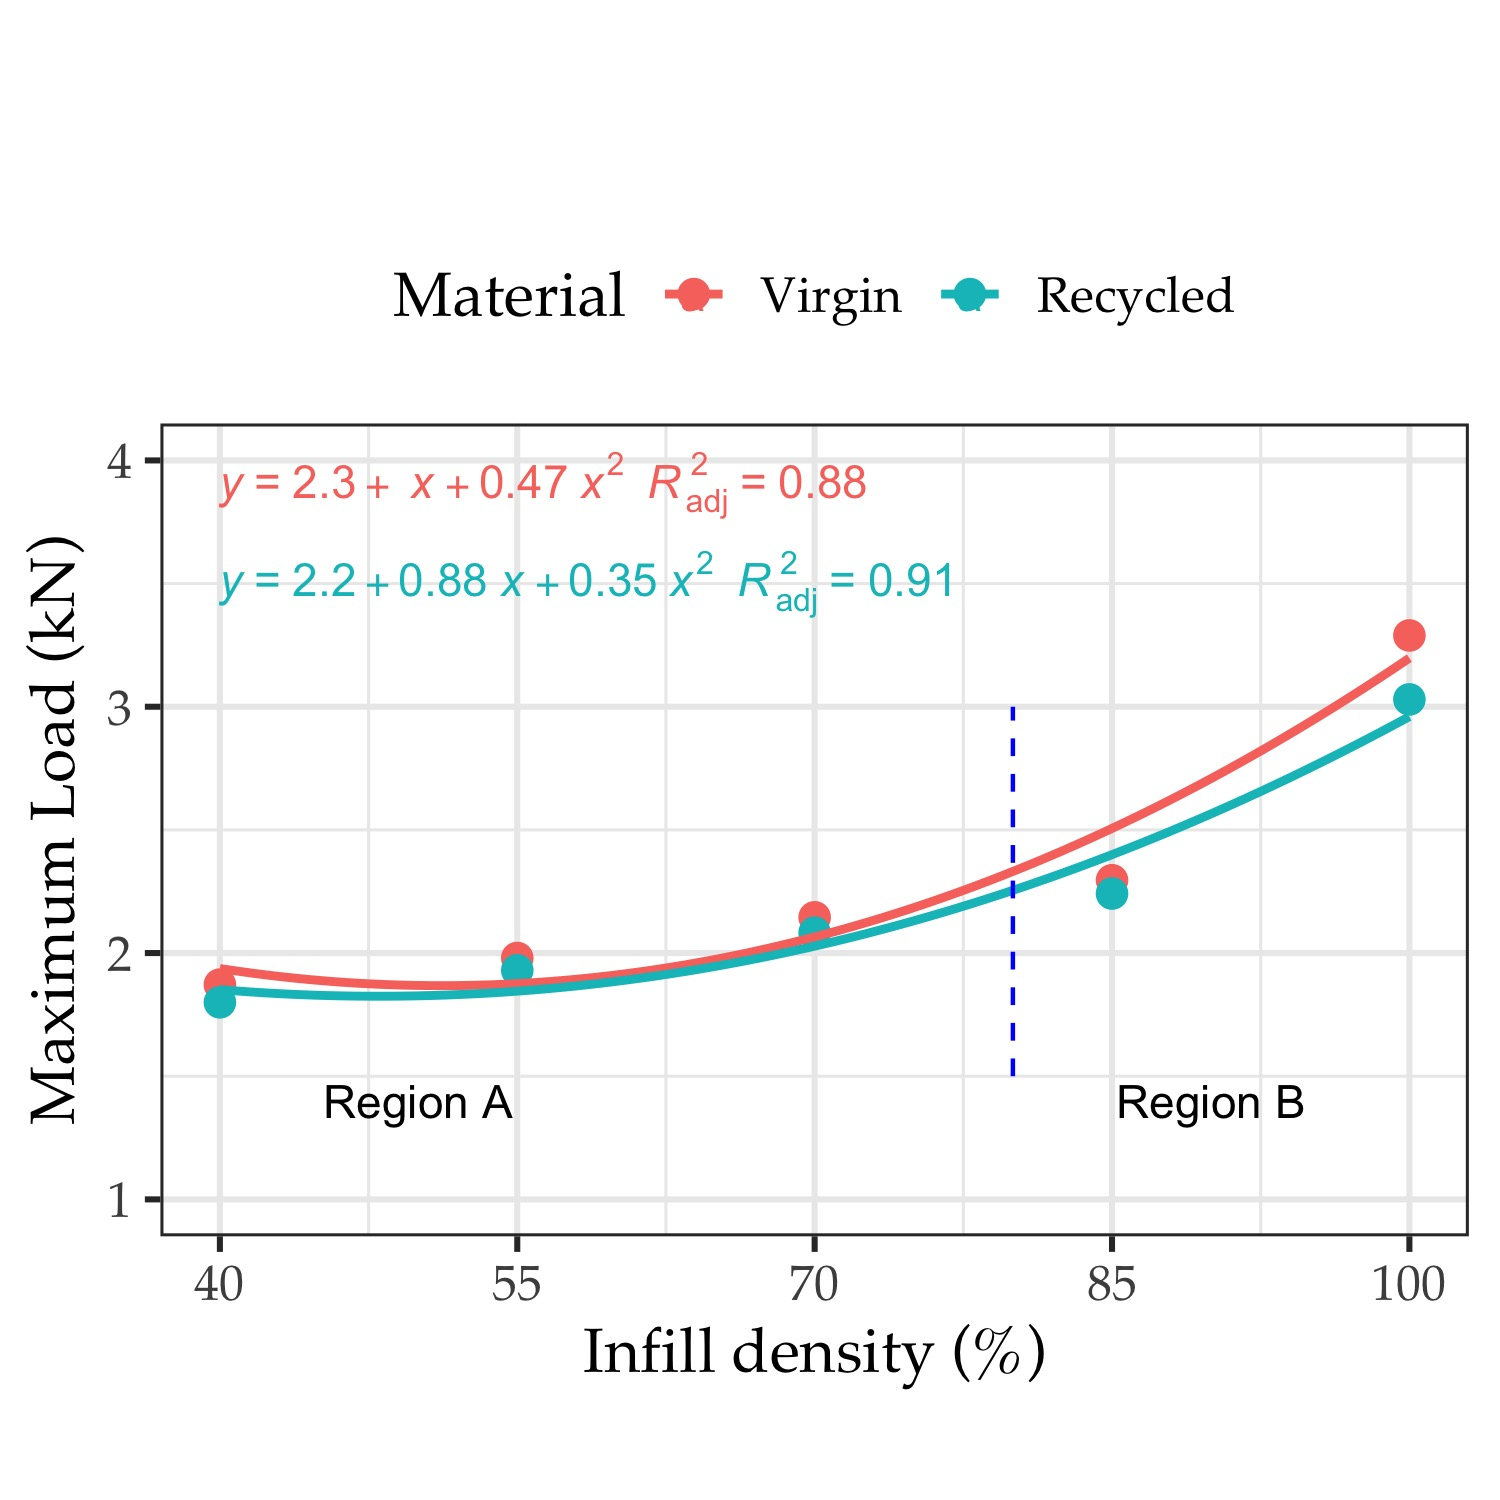
\includegraphics[width=0.49\linewidth]{Figures/Phase-2.jpg}%
\label{fig:phase2}}
\caption{Phase II: Tests to evaluate the evolution of significant the factor identified in Phase I.}
\end{figure}

Figure \ref{fig:probetas.phase2} shows the fracture of the specimens
tested in \emph{Phase II}. Regarding the fracture, the results were
similar to those of the \emph{Phase I} (i.e., more ductile behavior for
the recycled PLA specimens). The interesting element in this phase is
presented in Figure \ref{fig:phase2} where the maximum load versus
infill density for both virgin and recycled PLA is illustrated.

From the analysis of the Figure \ref{fig:phase2}, it is possible to
appreciate that there are two different regions. In the A region, which
is between infill densities from 40 to 80 \%, the slope of the curve
grows slowly with an approximately linear trend meaning that an increase
of the infill density provides a proportional increase in the mechanical
properties. On the other hand, as from 80\% of infill density, the
increase of the mechanical resistance becomes more pronounced, as
illustrated in the B region. Consequently, with a small increase of
infill density, the maximum load notably grows. Regarding the type of
material, it is clear that virgin PLA outperforms recycled PLA, but the
difference between them is limited. These results are in agreement with
studies on the comparison of the performance of recycled and virgin PLA
\citep{CruzSanchez2017} in which there was found a difference of about
10\% of the mechanical properties in the first recycling cycles.
However, the difference notably increased as the infill density
approached 100\%. The obtained results agree well with those presented
by \citet{Wang2020h}. In their study, the authors studied infill
densities of 20, 40, 60, 80 and 100\% and the evolution of the tensile
strength is similar to the one shown in Figure \ref{fig:phase2}.

Based on the results, it appears that a reduction from 100\% to 40\% of
the infill density implies a relatively limited reduction, in average
41.7\%, of the maximum load supported for both types of materials. This
is an interesting result that enables the creation of prototypes with
less material usage, without compromising the mechanical resistance.
Although the number of measured points is reduced, it is possible to
model the relation between the maximum load (y) versus the infill
density (x) for the two tested materials by means of polynomial
regressions that are plotted in the figure. The models may help to
anticipate the mechanical resistance of a part based on the selection of
the infill density. Based on the developed models, it is possible to
highlight that recycled PLA is a suitable substitute for virgin PLA
guaranteeing similar mechanical resistance. Moreover, by developing
models for the mechanical properties, it is possible to minimize the
material consumption for both virgin and recycled materials satisfying
the mechanical resistance requirements. Thus, by accurately knowing the
influence of the printing conditions on the mechanical resistance, it is
possible to advance towards sustainable manufacturing.

\hypertarget{phase-iii-study-on-the-printing-orientation}{%
\subsection{Phase III: Study on the printing
orientation}\label{phase-iii-study-on-the-printing-orientation}}

In this final phase, the main goal is to test the influence of the
building orientation according to the UNE 116005:2012
\citep{Garcia-Dominguez2020} standard. Five specimens for each of the
orientations (edgewise, horizontal and vertical) for both virgin and
recycled PLA were manufactured. The selected printing conditions were
infill density of 50\%, printing speed of 80 mm/s, tri-hexagonal infill
pattern and layer height of 0.3 mm, with the objective of limiting the
use of material and the time required for printing.

\begin{figure}[H]
\centering
\subfigure[Average of the load obtain for each build orientation.]{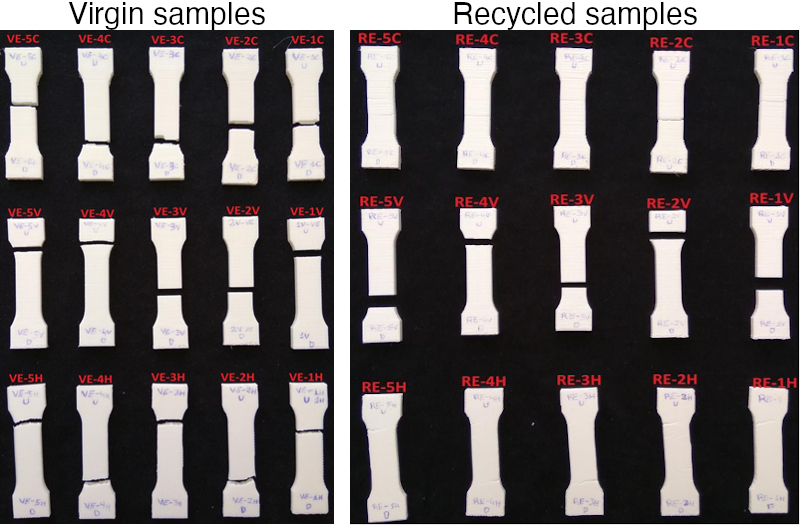
\includegraphics[width=0.8\linewidth]{Figures/Probetas-Fase-3.jpg}%
\label{fig:phase3a}}

\subfigure[Average of the load obtain for each build orientation.]{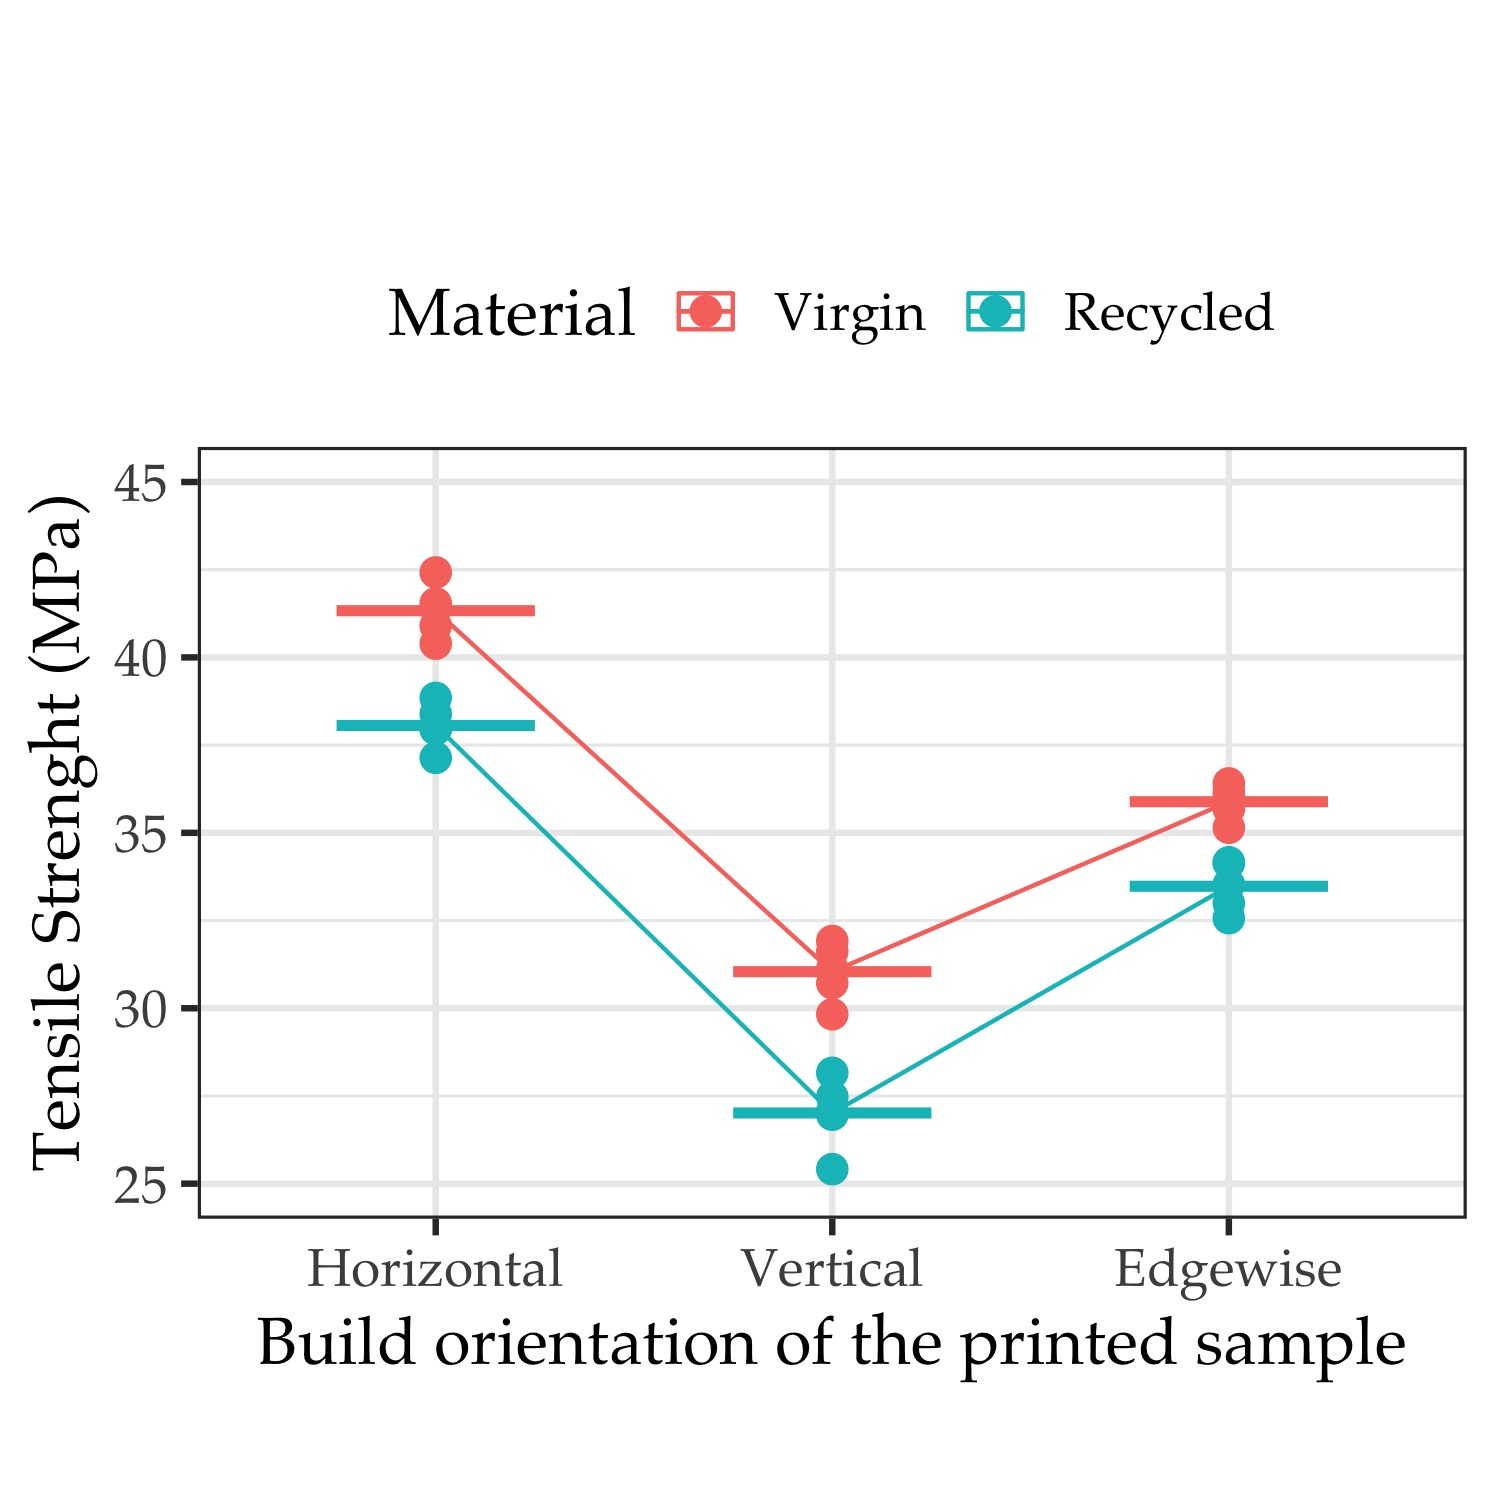
\includegraphics[width=0.6\linewidth]{Figures/Phase-3.jpg}%
\label{fig:phase3b}}
\caption{Phase III: Evaluation of the anisotropy.}
\end{figure}

Figure \ref{fig:phase3a} shows the images of the tested specimens
observing the same type of fracture as in the first two phases. It is
interesting to evaluate the reduction in the maximum load depending on
the type of material and orientation in which the specimens were
printed.

The Figure \ref{fig:phase3b} details the maximum load and the mean
values for the five specimens at each orientation. From the results, it
is clear that the horizontal orientation is the one that provided the
higher mechanical resistance, followed by the edgewise orientation.
Likewise, the virgin samples performed better than the recycled samples.

The vertical orientation provided the worse results due to the
deposition of the layers perpendicular to the tensile direction. These
results are in good agreement with those by \citet{Corapi2019} and
\citet{Wang2020h}. For the recycled material, there is a slight decrease
in the maximum load obtained from 6.71 to 13\% depending on the
orientation with respect to the virgin values. Particularly, the biggest
reduction of the load takes place in the vertical orientation with the
maximum decrease of 13 \%. However, the other two orientations are more
adequate for substituting the virgin material with the recycled material
with a limited reduction in mechanical resistance (6.71 to 7.93 \%).

\hypertarget{discussion-and-limits-of-the-results}{%
\section{Discussion and limits of the
results}\label{discussion-and-limits-of-the-results}}

\label{section:discussion}

One of the systemic problems of plastic waste relies on dependency of
the indiscriminate disposal of plastics, which carries multiple risks
because many plastic products contain additives that modify their
physico-mechanical properties, making it difficult the recycling/reuse
\citep{Wagner2020}. The use of 3D printing technology for prototyping
activities are not excepted of this societal issue. The main purpose of
this article is to assess to what extent the influence of the printing
parameters affects the tensile resistance of the printed parts. While a
large literature is focused on the optimization of the parameters for
obtaining functional printed objects using the 100\% of the printed
material, the approach made here is to observe the influence of a large
range of factors considered as critical within conventional printing
ranges. This type of approach is important because it enables designers
and users to use printing setups that are envisioned for prototypes
objects, being secure about the quality of the printed products.

One of the main results in this study relies on that that there is a
reduction about 41.7\% (in average) of the maximum load supported for
PLA (virgin and recycled) when the infill density changes from 100\% to
40\%. Moreover, it could be inferred from the results that an infill
density of 40\% retained 58.1\% of the mechanical resistance. This is a
relevant insight for prescriptions of minimal conditions for 3D
printing. Moreover, the use of recycled assets in the printing process
may be a relevant path, considering the current priorities of the
European Union on circular economy and carbon neutral strategies
ambitions \citep{Schwarz2021}. Also, there is a great development of
applications using distributed recycling approaches. For instance,
\citet{Nur-A-Tomal2020} presented a valuable example of waste-to-wealth
to use waste plastic toys retaining the original colour of waste plastic
to fabricate new products. Certainly more research is required to the
development of complete closed-loop case studies for prototyping
purposes based on material type validating technical, ecological and
economic feasibility \citep{CruzSanchez2020, Sauerwein2019}.

There are certain limitations to this work in the perspective of
materials and parameters tested. Definitely, the use of other materials
is needed to evaluate if the influence of the infill density and
recycled material are consequent with the results found. Moreover, other
factors are needed in order to consider the quality of a prototype.
Clearly, other key variables such as the aesthetic design, surface
finishing \citep{Jin2017}, dimensional accuracy are also key variables
to include for the printed objects in addition to the mechanical
resistance in the prototypes where the main goal is the user
acceptability \citep{Sauer2009, Sauer2010}. Nevertheless, this is an
ongoing research in which the main purpose is the statistical validation
of the minimal conditions to promote the use of recycled materials in
prototyping phases.

\hypertarget{conclusions}{%
\section{Conclusions}\label{conclusions}}

\label{section:conclusions}

The present study includes a comprehensive experimental program to
analyze the Fused Filament Fabrication process based on mechanical
resistance using virgin PLA and recycled PLA. The paper aims at
improving the sustainability of the 3D printing process, assessing the
technical feasibility of the substitution of virgin with recycled
filaments.

The printing conditions determined in a great manner the mechanical
resistance of the specimens. Specifically, the most influential factor
on the maximum load for both virgin and recycled PLA was the infill
density.\\
The influence of the infill density on the maximum load allowed
identifying two different regions: A, from 40 to 80\%, linear behavior
with a slight slope and, B, from 80 to 100 \%, the maximum load
increases notably to a greater extent. In general, the fracture of the
virgin material corresponded to that of a fragile material, while the
fracture of the recycled material showed a more ductile behavior.

The selected orientation for printing the specimens is of great
importance for the maximum load because of the anisotropy. In this
sense, the horizontal orientation allowed attaining a higher maximum
load, while the vertical orientation provided the lower value due to the
fact that no layers were deposited in the tensile direction. Our results
support the main argument on the substitution of virgin PLA with
recycled PLA based on the mechanical resistance for prototyping
purposes, advancing towards sustainable manufacturing. It was found that
using an infill density of 40\%, there is a retention of the 58.1\% of
the mechanical resistance. Despite recycled PLA offers a slightly lower
mechanical resistance, when possible, by properly selecting the printing
conditions (mainly, by the infill density and orientation) it could be
approximate the mechanical resistance to that of the virgin PLA.
Particularly, when using the edgewise and horizontal orientations, it is
possible to obtain maximum loads close to that of the virgin material
(from 3 to 8 \% lower).

\hypertarget{ackowledgements}{%
\section{Ackowledgements}\label{ackowledgements}}

The authors would like to thank the ``Mechanical and Energy
Engineering'' TEP 250 research group and to the Lorraine Fab Living
Lab\textsuperscript{\textregistered}. This research has received funding
from the European Union's Horizon 2020 research and innovation programme
under grant agreement No 869952.

\bibliographystyle{tfcad}
\bibliography{library.bib}




\end{document}
